%-------------------------------------------------------------------------------
\chapter{Mély tanuló alkalmazások fejlesztése}
%-------------------------------------------------------------------------------
A mély tanulás, konkrétabban a mesterséges neurális hálózatok gyors fejlődősét és részben népszerűségét a hozzá készített programozási keretrendszereknek köszönheti, melyek java szabad hozzáférésű. Ezek a keretrendszerek arra hivatottak, hogy támogassák a neurális hálózatok fejlesztését új programozási módszertant adva. Már létező programozási nyelvekre épülnek, leginkább python-ra. Ezekben a keretrendszerekben egyszerűen implementálhatunk neurális hálózatokat úgy, hogy egyfajta nyelvi eszközkészletet adnak neurális hálózatok definiálására.

\section{TensorFlow}
A Google mély tanulással kapcsolatos projektjeihez saját eszközöket fejleszt ki. Ilyen a TensorFlow (továbbiakban: TF) keretrendszer is, mely elsősorban mély tanuláshoz lett készítve, de elég flexibilis ahhoz, hogy egyéb numerikus számítást programozzunk általa. Több hardver típust is támogat, és képes elosztott számítás végrehajtására is -- ezalatt értem a többprocesszoros rendszereken és a számítógép-füzéreken történő futtatást. A TF az \emph{adatfolyam programozási} paradigmát valósítja meg. Ez a programozási modell jól illeszkedik a párhuzamos rendszerekhez. Eszközei \emph{adatfolyam gráfok} implementálását teszik lehetővé, amik a TF-ben távolról hasonlítanak a neurális hálózatok gráfjaira. Ezen felül leegyszerűsíti többdimenziós tömbök (\emph{tenzorok}) kezelését. Több programozási nyelvhez is biztosított API, így eszközei hívhatóak Python, JavaScript, C++ és Java kódokból, bár a dokumentáció felhívja a figyelmet, hogy a Python API szolgáltatja a legteljesebb eszközkészletet és tekinthető a legstabilabbnak.\cite{web:tfAPI} Jelenleg két, egymással részben kompatibilis stabil verziója van a TF-nak. A Google részletes dokumentációt biztosít a keretrendszerhez,\cite{web:tfGuide} illetve első megjelenésekor kiadott fehér könyv tervezési oldalról mutatja be a TensorFlow-t.\cite{tensorflow2015-whitepaper}

\begin{figure}[h]
	\begin{subfigure}{0.7\textwidth}
		\begin{lstlisting}[language=Python]
		import tensorflow as tf
		b = tf.Variable(tf.zeros([100]))
		W = tf.Variable(tf.random_uniform([784,100],-1,1))
		x = tf.placeholder(name="x")
		relu = tf.nn.relu(tf.matmul(W, x) + b)
		C = [...]
		s = tf.Session()
		for step in xrange(0, 10):
		input = ...construct 100-D input array...
		result = s.run(C, feed_dict={x: input})
		\end{lstlisting}\label{lst:TF}
		\caption{TensorFlow kódrészlet minta}
	\end{subfigure}
	\begin{subfigure}{0.25\textwidth}
		\centering
		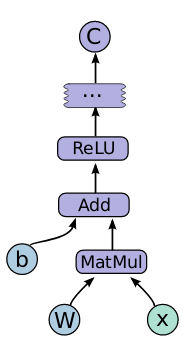
\includegraphics[width=0.9\columnwidth]{fig/TF_CompGraph}
		\caption{A kódban definiált számítási gráf}
		\label{fig:tfcompgraph}
	\end{subfigure}
	\caption{Számítási gráfok TensorFlowban}
\end{figure}

TensorFlowban a műveletek végrehajtásához műveleti csomópontokat kell definiálni, melyek egy-egy műveletet --~melyek a \verb|Operation| osztály példányai~-- valósítanak meg a számítási gráfban. Egy ilyen csomópontnak több bemenő, illetve kijövő éle lehet, melyek az átadott részszámításokat szimbolizálják --~a változók általánosan véve tenzorok a keretrendszeren belül. A \emph{Session} egységbe zárja a számításokat --~másként fogalmazva az \verb|Operation| és a \verb|Tensor| osztályok példányait~--, így a művelteket nem a gráfban implementációjában hajtódnak végre. Tehát a vezérlés külön van választva a program állapotától és a felhasználó az előbbit képes programozni. A TensorFlow új verziójában ez a megközelítés el lett rejtve, így például a \verb|outputs = session.run(f(placeholder), feed_dict={placeholder: input})| kifejezés helyett a sokkal rövidebb \verb|outputs = f(input)| használatos.

Több~processzoros rendszeren az egyes számításokat úgy oszthatjuk ki az eszközök között, hogy a megfelelő csomópontokat a célhardverhez társítjuk.
A kliens --~az alkalmazás, melyben a számítási-gráf definiálva lett~-- megszorításokat tehet a kiszolgálónak (dokumentációban:\emph{master}), hogy adott csomópontot --~vagy egy komplex munkafolyamatot~-- az eszközök mely csoportján lehet futtatni. Ezeket a megkötéseket a \verb|tf.device()| függvény paramétereként adhatjuk meg, és a megfelelő erőforrás-kezelővel tér vissza. A megkötések megadásának általános formája:\\
\verb|/job:<JOB_NAME>/task:<TASK_INDEX>/device:<DEVICE_TYPE>:<DEVICE_INDEX>|
ahol,
\begin{description}
	\item[JOB\_NAME] egy betűvel kezdődő alfanumerikus karaktersorozat,
	\item[DEVICE\_TYPE] az eszköz típusa (például GPU vagy CPU),
	\item[TASK\_INDEX] egy nemnegatív egész szám, ami a <JOB\_NAME> egy feladatának sorszáma,
	\item[DEVICE\_INDEX] egy nemnegatív szám, ami több hasonló típusú eszköz esetén a megfelelő eszköz sorszáma.
\end{description}
Példaképpen a képbetöltést és mátrix szorzat számítást az alábbi módon tudjuk szétosztani az alaplapi és a grafikus processzor között:\cite{github:TF1-guide_distribution}
\begin{lstlisting}[language=Python]
with tf.device("/device:CPU:0"):
    img = tf.decode_jpeg(tf.read_file("img.jpg"))

with tf.device("/device:GPU:0"):
    result = tf.matmul(weights, img)
\end{lstlisting}

A TensorFlow tehát egy nagyon rugalmas és jól skálázható keretrendszer, azonban a programozóra hárítja a neurális hálózat rétegeinek pontos implementációját, továbbá párhuzamos rendszerek esetén a számítási feladatok szétosztását. Születtek ezért olyan eszközök, melyek a TF ,,előtétjeként'' igyekeznek megszabadítani a felhasználót a hosszadalmas és aprólékos fejlesztéstől.

\section{Keras}
A Keras egy python nyelven írt programkönyvtár, vagy ahogy önmagát hívja ''magas szintű neurális hálózat API''\cite{web:Keras}. Fejlesztésébe François Chollet kezdett bele. Érdekessége, hogy más olyan keretrendszerekkel együttesen használható, amelyek a Keras-hoz hasonlóan magas absztrakciós szinten biztosítják a hálózatok implementálását, mint például a TensorFlow.
%A Keras-ról szerzett tudásom javát Chollet könyvéből és a keretrendszer dokumentációjából szereztem.\cite{Chollet}\cite{web:Keras}.
Chollet könyve részletesen bemutatja a keretrendszer használatát, továbbá nyíltan hozzáférhető annak dokumentációja is.\cite{chollet}\cite{web:Keras}
\begin{figure}[h]
	\centering
	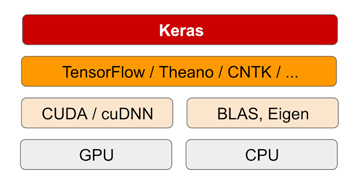
\includegraphics[width=0.5\linewidth]{fig/keras_software_stack}
	\caption{Keras szoftver rendszer\protect\footnotemark}
	\label{fig:kerassoftwarestack}
\end{figure}
\footnotetext{Forrás:\protect\cite{chollet}}

\subsection{Neurális hálózat definiálása}
Keras-ban egy neurális hálózatot \emph{model}-nek hívunk (gyakran máshol is így neveznek egy konkrét neurális hálózatot). Egy \emph{model} létrehozásához a \verb|Keras.models| modulban definiált metódusokkal lehetséges. A keretrendszerben az adatokat tenzorokként kell reprezentálnunk, ezért érdemes a \emph{numpy}\footnote{lásd:\url{https://numpy.org/}} nevű python csomaggal együtt használni. A keretrendszer tetszőleges alakú tenzorokat képes kezelni, tehát nincs megkötés arra vonatkozóan, hogy egy réteg bemenete vektor, mátrix vagy kiterjedtebb struktúrában -- magasabb dimenziójú tenzorban -- szerepeljen. A következő kódokban szeretném szemléltetni a Keras használatának módját.

A \ref{lst:defLayers} kód egy két rétegből álló neurális hálózat definiálását mutatja be.
\begin{minipage}{\textwidth}
\begin{lstlisting}[language=Python, caption=Neurális hálózat rétegeinek definiálása]
from keras import models
from keras import layers

network = models.Sequential()
network.add(layers.Dense(15, activation='relu', input_shape=(784,)))
network.add(layers.Dense(10, activation='softmax'))
\end{lstlisting}\label{lst:defLayers}
\end{minipage}
A kód 4. sorában inicializáljuk a hálózatot, az utána következő sorokban új neuron rétegeket adunk a hálózathoz. Kerasban különböző előre definiált rétegkapcsolatok vannak. Itt a \verb|layers.Dense| osztály egy a szomszédos rétegekkel teljesen összekapcsolt réteget implementál --~azaz egy neuron az előző réteg összes neuronjához kapcsolódik.
A réteg bemenetként $28 \times 28 = 784$ elemű vektorokból álló mátrixot tud fogadni, másik dimenziója nem meghatározott. Ez a kötegelt adatfeldolgozás szempontjából fontos, tehát a bemeneti vektorok folyamát egyik dimenziójában nem meghatározott méretű tenzorral definiáljuk. A réteg kimenete egy 15 dimenziós vektor. A következő réteg pedig 10 elemű tömböt állít el. Megfigyelhető, hogy nem adtuk meg a bemenet méretét, ugyanis a keretrendszerben ez implicit módon rendelődik a réteghez. 

Mindkét réteghez tartozik egy \emph{activation} paraméter, mely string típus kell legyen, és a réteg neuronjaihoz tartozó aktivációs függvényt adja meg. A példában a \verb|'relu'| és \verb|'softmax'| string a \ref{sec:fuggvenyek-algoritmusok} fejezet \eqref{eq:relu} és \eqref{eq:softmax} függvényére utal, azaz ezen bemeneti paraméterek esetén olyan \verb|Dense| objektum jön létre, mely ilyen aktivációs függvényekkel rendelkező neuron réteget valósít meg.

A \verb|Keras.layers| modulban A \verb|Dense| osztályon kívül implementálva vannak konvolúciós, összefésülő, zaj, stb. rétegek, melyek a fenti módon tetszés szerint egymásra szervezhetőek a keretrendszerben, így szinte tetszőleges hálózat alakítható ki.

\subsection{Hálózat betanítása és betanított hálózat futtatása}
\label{subsect:inference}
A megalkotott hálózatot a \verb|network| objektum definiálja. Hogy tanítható legyen el kell látni egy optimizálóval és egy veszteségfüggvénnyel, melyek együtt adják a hálózatot betanító algoritmust. A \verb|compile()| metódus ,,összerakja'' a neurális hálózatot a betanítóval, a \verb|fit()| pedig elvégzi a tanítást, és \emph{epoch}-ok számának megfelelő méretű tömböket tartalmazó objektum referenciájával tér vissza, mely tömbökben össze vannak gyűjtve a veszteségfüggvény értékei és a felhasználói metrikák eposzonként. 
\begin{minipage}{\textwidth}
\begin{lstlisting}[language=Python,caption=Hálózat betanítása]
network.compile(optimizer = 'sgd',
loss = 'mean_squared_error',
metrics = ['acc'])

history = network.fit(train_datas,
						train_labels,
						epochs=20,
						batch_size=512)
\end{lstlisting}\label{lst:fitNetwork}
\end{minipage}

A \verb|train_datas| és \verb|train_labels| a tanítókészletet alkotó minták és azok címkéi, a várt kimeneti értékek (ezek elemszáma kötelezően meg kell egyezzen). A \emph{batch\_size} paraméter a \emph{mini batch-ok} méretét adja, ami az egy \emph{epoch}-ban egyszerre feldolgozandó adatokat jelenti. A betanítás végén a \verb|network| egy \emph{betanított}, a célfeladat megoldására felhasználható neurális hálózat lesz. Alkalmazásához a \verb|predict()|metódus használatos, mely a paraméterként megadott bemeneti adatokhoz tartozó predikciókkal tér vissza.
\begin{minipage}{\textwidth}
\begin{lstlisting}[language=Python, caption=Az eszközre töltött hálózat futtatása az adatokon]
	result = network.predict(datas)
\end{lstlisting}
\end{minipage}

\subsection{Hatékonyságvizsgálat}

A tanítás felügyeletére a tanításhoz rendelkezésre álló adatok egy részét külön kell választanunk a tanítókészlettől. Ez a készlet lesz a validálási készletünk, mellyel minden tanítási ciklus végén leellenőrizzük, hogy hogyan teljesít a hálózat olyan adaton, amit még ,,nem látott''. A validálást Keras-ban megtehetjük a tanítással egy lépésben, a \verb|fit()| algoritmussal, ha a \verb|validation_data| opcionális paraméterének megadunk egy \verb|(data, label)| \verb|tuple| típusú változót. Ekkor a metódus olyan referenciával tér vissza (\ref{lst:fitNetwork}~kódrészletben ez a \verb|history|), melyen keresztül a tanítási és validálás statisztikák is beolvashatóak. A \ref{subsect:inference}~szakaszban említett metrikák a validálási folyamathoz is rögzítve lesznek. 
\begin{figure}[H]
	\centering
	\begin{subfigure}{0.45\textwidth}
		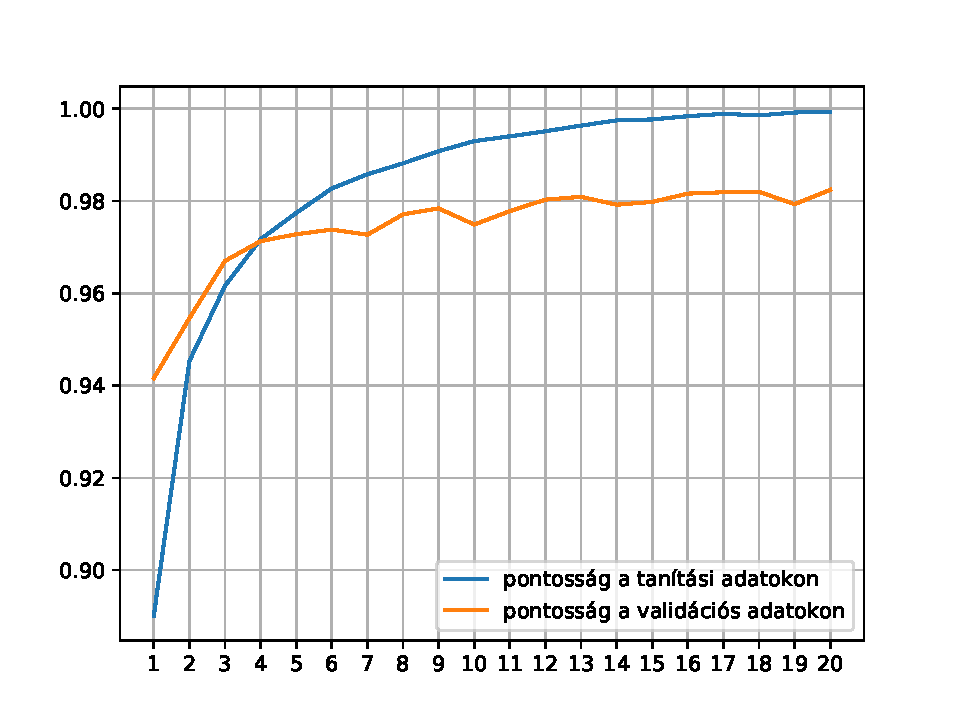
\includegraphics[width=\textwidth]{fig/accuracy.pdf}
		\label{fig:plotacc}
	\end{subfigure}
	\quad
	\begin{subfigure}{0.45\textwidth}
		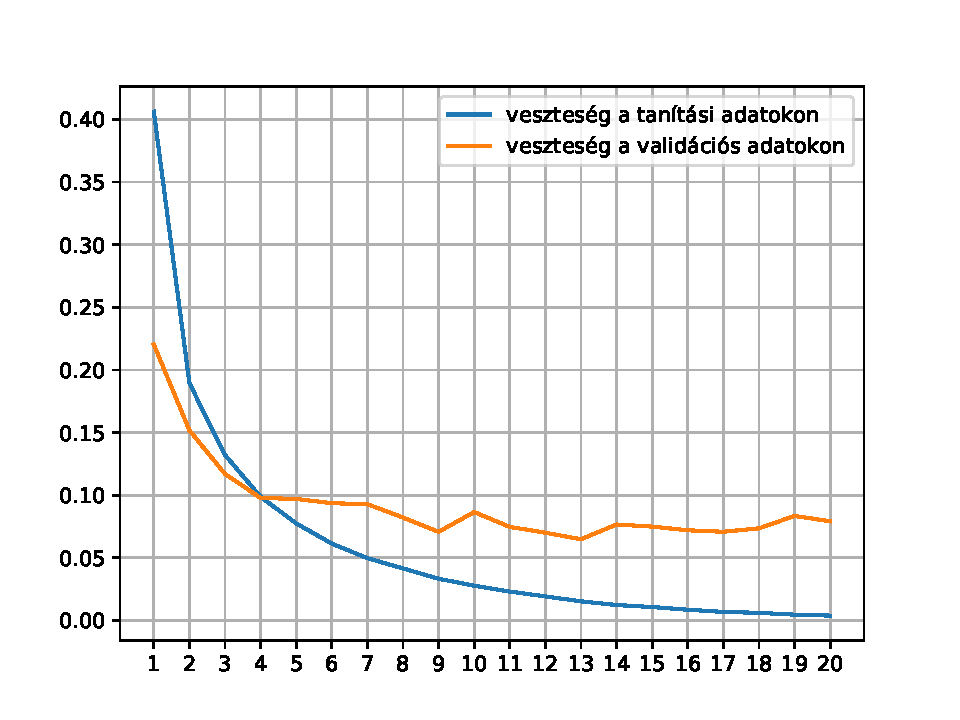
\includegraphics[width=\textwidth]{fig/loss.pdf}
		\label{fig:plotloss}
	\end{subfigure}
	\caption{Példa kimutatás a Keras által gyűjtött statisztikákról}
\end{figure}